\chapter{Grundlagen}
\label{ch:grundlagen}
Das folgende Kapitel beschreibt elementare Grundlagen, die zum Verständnis der nachfolgenden Kapitel notwendig sind. Der
erste Abschnitt befasst sich mit den verwendeten Maschinen und Komponenten der Robert Bosch Packaging GmbH.

Der zweite Teil widmet sich der Künstlichen Intelligenz und den verschiedenen Untergruppen und Ausprägungen, welche in
diesem Bereich existieren. Es wird dabei unter anderem auf die Konfiguration der Produkte und Laufzeitumgebungen
eingegangen. Außerdem werden hier die Programme und Konzepzte behandelt, welche in dieser Arbeit benötigt werden.

Im letzten Teil des Kapitels folgt die Beschreibung einer Designidee bei Smartphone-Apps, allgemeine Konzepte der
Softwareentwicklung und ein Framework zum Entwickeln von Webseiten.

\section{Bosch KWE Waage}
Was ist die Bosch KWE Waage. Parameter der Waage definieren.
\colorbox{yellow}{Hier fehlt was}

\section{Künstliche Intelligenz}
Was ist künstliche Intelligenz?

\colorbox{yellow}{Hier fehlt was}

In Abbildung~\ref{fig:grundlagen_artificialintelligence} auf Seite~\pageref{fig:grundlagen_artificialintelligence} ist
die Einordnung der Künstlichen Intelligenz in ihre Untergruppen ersichtlich. Dabei handelt es sich um eineigene Darstellung
nach CodesofInterest\footnote{https://www.codesofinterest.com/2016/11/difference-artificial-intelligence-machine-learning-deep-learning.html}.

\begin{figure}[h]
    \centering
    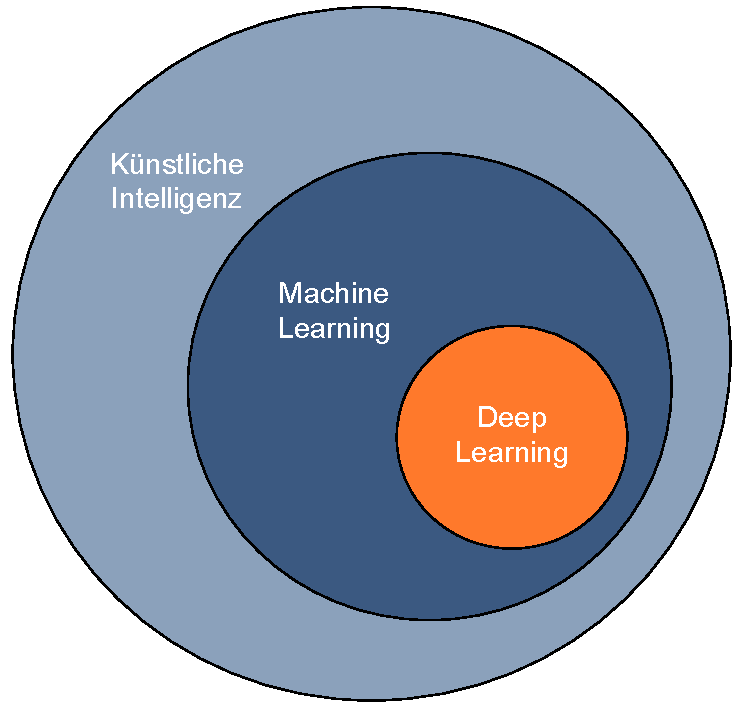
\includegraphics[scale=0.6]{images/kapitel_2/kuenstliche_intelligenz.pdf}
    \caption{Unterscheidung der Künstlichen Intelligenz}
    \label{fig:grundlagen_artificialintelligence}
\end{figure}

\section{Machine Learning}
Was ist Machine Learning?
\colorbox{yellow}{Hier fehlt was}

\subsection{Algorithmen}
Welche Algorithmen gibt es dafür
\colorbox{yellow}{Hier fehlt was}

\subsection{Bewertungskriterien}
Welche Bewertungskreterien gibt es
\colorbox{yellow}{Hier fehlt was}

\subsection{Klassifikation}
Welche Klassifikationen gibt es
\colorbox{yellow}{Hier fehlt was}

\subsection{Deep Learning}
Was ist Deep Learning
\colorbox{yellow}{Hier fehlt was}

\subsection{Neuronale Netze}
Was ist ein Neuronales Netz
\colorbox{yellow}{Hier fehlt was}

\section{Cloud}
Der Begriff Cloud hat sich als Kurzform des Cloud Computing etabliert und versteht das Zusammenspiel von mehreren Servern.
Die Server übernehmen Aufgaben, wie etwa die Datenspeicherung oder komplizierte Programmabläufe. Dabei erkennt der
Cloud-Nutzer nicht, wie viele Server hinter der Cloud stecken oder wo diese sich befinden.

Selbst wenn ein Server ausfällt, hat dies keine Auswirkungen auf das gesamte System, da die Anfragen und Aufgaben auf
die anderen Systeme umgeleitet werden.

Die Cloud zeichnet sich nach NIST~\cite{online_grundlagen_cloud_nist} und~\cite{online_grundlagen_cloud_computing} durch
fünf wesentliche Eigenschaften aus:

\begin{itemize}
    \item \textbf{On-Demand Self Service} \\
    Registrierte Nutzer können Resourcen selbstständig instantiieren und konfigurieren.
    \item \textbf{Broad Network Access} \\
    Der Zugriff kann von verschiedenen Endgeräten erfolgen.
    \item \textbf{Resource Pooling} \\
    Alle Resourcen des Anbieters werden gebündelt und nach Bedarf den Nutzern zugewiesen.
    \item \textbf{Rapid Elasticity} \\
    Kapazitäten können nach Bedarf skaliert werden und stehen schnell und dynamisch zur Verfügung.
    \item \textbf{Measured Service} \\
    Es existiert eine automatische Kontrolle der Ressourcen durch einen Zähler, welcher die Transparenz für den
    Anbieter und den Benutzer ermöglicht.
\end{itemize}

Auf dem Markt existieren etliche Cloud-Anbieter. Im folgenden wird auf drei der Top 10 größten Anbieter und deren Lösungen
im Bereich künstliche Intelligenz eingegangen (Siehe dazu~\cite{online_grundlagen_cloud}).

\subsection{Microsoft Azure}
Was ist Azure
\colorbox{yellow}{Hier fehlt was}

\subsubsection{Azure Machine Learning Studio}
Beschreiben des Tools von Azure für Machine Learning
\colorbox{yellow}{Hier fehlt was}

\subsection{Amazon Web Services}
Was ist AWS
\colorbox{yellow}{Hier fehlt was}

\subsubsection{Amazon Machine Learning}
Beschreiben des Tools von AWS für Machine Learning
\colorbox{yellow}{Hier fehlt was}

\subsection{IBM Cloud (ehemals Bluemix)}
Bluemix ist die von IBM entwickelte Cloud-Platform. Über Bluemix greifen Entwickler auf mehr als 160 Cloud-Services zu,
um mobile Apps und Webanwendungen zu entwickeln. In Bluemix gibt es zahlreiche Analysewerkzeuge sowie Services von
Drittanbietern. Mit Watson Analytics lassen sich beispielsweise intelligente Systeme realisieren, die Daten kognitiv
(also selbstlernend, ohne für die Problemlösungen programmiert zu sein) auswerten und für die Entscheidungsfindung
aufbereiten.

Bluemix unterstützt diverse integrierte DevOps-Dienste, um Cloud-Anwendungen zu erstellen, auszuführen, bereitzustellen
und zu verwalten. Die Entwicklerplattform basiert auf der Technologie von Cloud Foundry und läuft auf IBMs
Softlayer Cloud Infrastruktur. Sie unterstützt mehrere Programmiersprachen, einschließlich Java, Node.js, Go, PHP,
Python, Ruby Sinatra, Ruby on Rails und kann auch andere Sprachen wie Scala durch den Einsatz von Buildpacks
unterstützen~\cite{online_grundlagen_bluemix}.

Weitere Informationen üer Bluemix können auf der Webseite\footnote{https://bluemix.net} gefunden werden.

\subsubsection{Watson Studio}
Was ist das und was kann man damit machen
\colorbox{yellow}{Hier fehlt was}

\subsubsection{Cloud Object Storage}
Was ist das
\colorbox{yellow}{Hier fehlt was}

\subsubsection{Apache Spark}
Was ist das
\colorbox{yellow}{Hier fehlt was}

\subsubsection{API Connect}
Was ist das
\colorbox{yellow}{Hier fehlt was}

\subsubsection{Toolchain}
Bei einer Toolchain handelt es sich um ein Tool zur Verwaltung von Entwicklung, Bereitstellung sowie Üerwachung einer
Anwendung. Nach der Einrichtung einer Toolchain stehen verschiedene Services zur Verfügung, welche zum Beispiel eine
Integration zu einem GitHub-Projekt ermöglichen.

Mit einer eingerichteten Toolchain und einem verbundenen Git-Repository kann der Quelltext gebaut und auf einem System
installiert werden. Bei der Toolchain handelt es sich unter anderem um ein \textit{Continuous Integration}-Tool (kurz CI)
(Mehr unter~\cite{online_grundlagen_toolchain}).

\section{TensorFlow.js}
Was ist TensorFlow und wie nutzt man das. Es geht hier dann um TensorFlow.js
\colorbox{yellow}{Hier fehlt was}

\section{Angular}
Was ist Angular und was macht man damit
\colorbox{yellow}{Hier fehlt was}

\subsection{Model-View-Controller}
Model-View-Controller (kurz MVC) wurde um 1978 von Xerox entwickelt und es handelt sich dabei um eine Architektur von
Programmen.

In MVC wird eine Anwendungskomponente in drei Teile zerlegt. In das oberflächenunabhängige \textit{Model}, das für die
Ausgabe zuständige \textit{View} und den für die Interpretation von Eingabeereignissen zuständigen \textit{Controller}.

Der Controller ist die Steuerungseinheit, das Model der Anwendungskern und die View der Darsteller bzw. die Ansicht der
Anwendung. Ein View zusammen mit seinem Controller wird hier auch als eine Oberfläche bezeichnet (Mehr hierzu
unter~\cite{book_grundlagen_mvc}).

Es gibt zahlreiche Frameworks, welche das MVC-Patern umsetzen. AngularJS ist einer der bekanntesten Vertreter.

\subsection{Angular-Material}
Was kann man damit machen
\colorbox{yellow}{Hier fehlt was}

\subsection{ngx-restangular}
Was bringt die Library
\colorbox{yellow}{Hier fehlt was}

\subsection{Observable}
Was ist das für ein pattern?
\colorbox{yellow}{Hier fehlt was}

\subsection{Promise}
Was ist das für ein pattern
\colorbox{yellow}{Hier fehlt was}

\subsection{flex-layout}
Was kann man damit erreichen
\colorbox{yellow}{Hier fehlt was}

\section{REST}
REST-API steht für Representational State Transfer - Application Programming Interface. Diese Interfaces machen den
Austausch von Informationen uüber unterschiedliche Systeme möglich. Im Zeitalter verteilter Systeme und Cloud-Computing
trifft man oft auf unterschiedliche Systeme, welche den Einsatz von REST-API notwendig machen.

Man spricht bei REST-API auch von der Maschine-Maschine-Kommunikation, da die verschiedenen Systeme und Geräte
zusammengebracht werden und gewissermaßen die gleiche Sprache sprechen.

Mit REST-API ist es möglich geworden, Informationen und Aufgaben auf verschiedene Systeme zu verteilen und diese mit der
Hilfe von HTTP-Requests anzufordern. Jeder HTTP-Request setzt sich aus dem Endpoint und den entsprechenden Parametern
zusammen~\cite{online_grundlagen_rest}.

\section{Cloud Foundry}
Cloud Foundry ist eine Open Source Platform as a Service (PaaS) Lösung. Mit Hilfe von Cloud Foundry können Entwickler
ihre Anwendungen bauen, hochladen und ausführen. Ein großer Vorteil von Cloud Foundry ist die nahezu grenzenlose
Skalierbarkeit~\cite{online_grundlagen_cf}.

Die Skalierbarkeit wird durch die Container-Architektur erreicht. Jeder Container beinhaltet eine eigene Anwendungsinstanz.
Dabei wird sowohl eine horizontale als auch eine vertikale Skalierung unterstützt.

Bei der horizontalen Skalierung werden zusätzliche Container gestartet oder gestoppt und ein Load Balancer vor die
Container geschaltet. Bei der vertikalen Skalierung werden jeder Instanz individuell z.B. mehr oder weniger Arbeitsspeicher
zugeteilt.

Jede Cloud Foundry Instanz besitzt eine IPV4-Adresse wodurch es mittels A-Record (Zuordnung eines DNS-Namens zu IP-Adresse)
möglich ist, eine eigene Domain mit der Anwendung zu verknüpfen.

\section{Version Control (Git)}
Was ist das und für was ist das gut
\colorbox{yellow}{Hier fehlt was}

\section{Node Package Manager (npm)}
Was ist das und für was ist das gut
\colorbox{yellow}{Hier fehlt was}

\section{Mockups}
Was bringt sowas
\colorbox{yellow}{Hier fehlt was}

\section{TypeScript}
Was hat man da für Vorteile und was ist das
\colorbox{yellow}{Hier fehlt was}

\section{WebView}
Bei WebView handelt es sich um ein Android- und iOS-Layout, das Webseiten darstellen kann. Über Schnitstellen werden
Informationen wie Webseite, URL und Größe üergeben. Das Laden, das Anzeigen und die Interaktion mit der Webseite üernimmt
das Layout selbstständig.

Das Layout steht sowohl unter Android als auch iOS in den frühesten Versionen zur Verfügung (Weitere Informationen
unter~\cite{online_grundlagen_webview}).